\documentclass{beamer}
%
% Choose how your presentation looks.
%
% For more themes, color themes and font themes, see:
% http://deic.uab.es/~iblanes/beamer_gallery/index_by_theme.html
%
\mode<presentation>
{
  \usetheme{Madrid}      % or try Darmstadt, Madrid, Warsaw, ...
  \usecolortheme{beaver} % or try albatross, beaver, crane, ...
  \usefonttheme{default}  % or try serif, structurebold, ...
  \setbeamertemplate{navigation symbols}{}
  \setbeamertemplate{caption}[numbered]
} 

\usepackage[english]{babel}
\usepackage[utf8x]{inputenc}
\usepackage{xcolor}
\usepackage{mathtools}
\usepackage{listings}
\usepackage{xcolor}

\lstset{% This applies to ALL lstlisting
	%backgroundcolor=\color{yellow!10},%
	%numbers=left, numberstyle=\tiny, stepnumber=2, numbersep=5pt,%
}%

% Applies only when you use it
\lstdefinestyle{ANTLR}{
	basicstyle=\footnotesize\ttfamily\color{magenta},%
	breaklines=true,%                                      allow line breaks
	moredelim=[s][\color{green!50!black}\ttfamily]{'}{'},% single quotes in green
	moredelim=*[s][\color{black}\ttfamily]{options}{\}},%  options in black (until trailing })
	commentstyle={\color{gray}\itshape},%                  gray italics for comments
	morecomment=[l]{//},%                                  define // comment
	emph={%
		STRING%                                            literal strings listed here
	},emphstyle={\color{blue}\ttfamily},%              and formatted in blue
	alsoletter={:,|,;},%
	morekeywords={:,|,;},%                                 define the special characters
	keywordstyle={\color{black}},%                         and format them in black
}

\title[Theory of languages]{Introduction to theory of languages}
\author{Patryk Kiepas}
\institute{MINES ParisTech \& AGH}

\date{\today}

\begin{document}


% --------------------------------------------------------------------- %
\begin{frame}
  \titlepage
\end{frame}

\section{Introduction}

% --------------------------------------------------------------------- %
\begin{frame}{Course plan}

\begin{enumerate}
\item Saturday, 25th of February 2017 -- lecture
\begin{itemize}
\item Languages
\item Grammars
\end{itemize}
\item Saturday, 4th of March 2017 -- lecture
\begin{itemize}
\item Parsing
\item ANTLR
\end{itemize}
\item Saturday, 11th of March 2017 -- exercises
\begin{itemize}
\item Grammars and languages
\item ANTLR
\end{itemize}
\item Saturday, 25th of March 2017 -- exercises
\begin{itemize}
\item ANTLR
\end{itemize}
\item Exam
\end{enumerate}

\end{frame}

% --------------------------------------------------------------------- %
\begin{frame}[fragile]{Additional informations}
\begin{alertblock}{Any questions?}
Ask by mail: \verb|kiepas@agh.edu.pl|
\end{alertblock}

\begin{alertblock}{Course web-page}
\verb|http://home.agh.edu.pl/~kiepas| $\rightarrow$ \textbf{Teaching} $\rightarrow$ \textbf{Introduction to theory of languages (2017)}
\end{alertblock}
\end{frame}

% --------------------------------------------------------------------- %
\begin{frame}{Outline}
	\tableofcontents
\end{frame}

\section{Theory}

\subsection{Languages}

% --------------------------------------------------------------------- %
\begin{frame}{Introduction}

\begin{block}{Linguistics}
Scientific study of languages. Involves analysis of language:
\begin{itemize}
\item \textit{form} -- language evolution and task
\item \textit{context} -- environment of language usage
\item \textit{semantics} -- the meaning of the language
\end{itemize}
\end{block}

\begin{block}{Some important aspects}
\begin{itemize}
\item Phonetics
\item Articulation
\item Perception
\item Acoustic features
\item Morphology
\item Syntax
\end{itemize}
\end{block}

\end{frame}

% --------------------------------------------------------------------- %
\begin{frame}{Language types}
\begin{enumerate}
\item Natural languages
\begin{itemize}
\item \textit{Ordinary} -- evolves naturally in humans without planning
\item \textit{Controlled} -- a restricted subset of natural language in order reduce or eliminate ambiguity and complexity
\end{itemize}
\item \textbf{Artificial languages}
\begin{itemize}
\item \textit{Constructed} (planned \textit{a priori} or \textit{a posteriori})
\begin{itemize}
\item Engineered languages -- experiments in \textit{logic}, \textit{philosophy}, \textit{linguistics}
\item Auxiliary languages -- international communication (e.g. Esperanto, Ido,  Interlingua)
\item Artistic languages -- aesthetic pleasure or humorous effect (e.g. Klingon)
\end{itemize}
\item \textit{\textbf{Formal}}
\begin{itemize}
\item Computer programming languages (e.g. Java, Haskell, C, C++, Ruby)
\item Files and formats descriptions (e.g. YAML, JSON, XML)
\end{itemize}
\end{itemize}
\end{enumerate}
\end{frame}

% --------------------------------------------------------------------- %
\begin{frame}{Description of natural languages}

\begin{block}{A really small bit of history}
\begin{itemize}
\item In the late 1950's Noam Chomsky tried to describe natural languages
\item Important paper:  \textit{"Three models for the description of language"}, Noam Chomsky (1956).
\item In a result of his research two disciplines originated:
\begin{enumerate}
\item \textbf{\textit{Theory of formal grammars}}
\item \textit{Generative (transformational) grammars}
\end{enumerate}
\end{itemize}
\end{block}

\begin{figure}
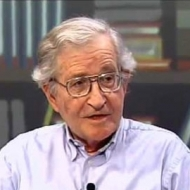
\includegraphics[width=0.2\textwidth]{img/noam_2.jpg}
\caption{\label{fig:your-figure}Professor of Linguistics (Emeritus) at MIT, Cambridge}
\end{figure}

\end{frame}

% --------------------------------------------------------------------- %
\begin{frame}{Description of natural languages}

\begin{block}{What we know now?}
\begin{itemize}
\item Description of natural languages is \textbf{hard}
\item Description of any natural languages might be \textbf{impossible}
\end{itemize}
\end{block}

\begin{block}{Why this is important?}
\begin{itemize}
\item Better understanding of language creation processes
\item More insights into functioning of our brain
\item \textbf{Natural language processing (NLP)}
\begin{itemize}
\item Translations (e.g. Google Translator)
\item Synthesis (e.g. speech generation)
\item Perceiving (e.g. robots, voice-control)
\end{itemize}
\end{itemize}
\end{block}

\end{frame}

% --------------------------------------------------------------------- %
\begin{frame}{Description of formal languages}

\begin{alertblock}{Result}
Description of natural languages help us describe an artificial (formal) ones
\end{alertblock}

\begin{block}{Programming languages}
\begin{itemize}
\item Protocol for communication with the computer
\item Performing operations and computations
\item Interpretation and execution
\item Compilation
\item Static code analysis
\end{itemize}
\end{block}

\begin{block}{Data formats}
\begin{itemize}
\item Structured data
\item Interchangeable model for communication and data transmission
\end{itemize}
\end{block}

\end{frame}

% --------------------------------------------------------------------- %
\begin{frame}{Alphabet}

\begin{block}{Alphabet}
A set $\Sigma$ of available symbols, the simplest elements in the language
\end{block}

\begin{exampleblock}{Examples}
\begin{itemize}
\item binary alphabet $\{0, 1\}$
\item decimal numbers $\{0,1,2,3,...,9\}$
\item Latin alphabet $\{a,b,c,d,...,z\}$
\item Cyrillic
\end{itemize}
\end{exampleblock}

\begin{figure}
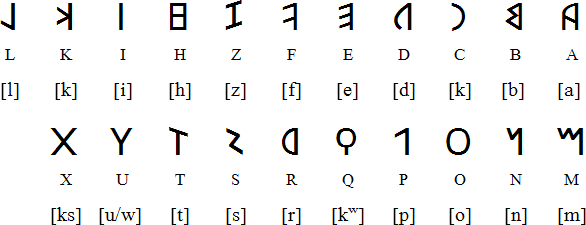
\includegraphics[width=0.5\textwidth]{img/latin_archaic.png}
\caption{\label{fig:latin_archaic}Ancient Latin alphabet}
\end{figure}

% --------------------------------------------------------------------- %
\end{frame}

\begin{frame}{Word (I)}
\begin{block}{Word}
Word $w$ is a sequence of $N$ symbols $w = x_1x_2...x_N$ where $x_i\in\Sigma$ \\ (e.g. $010110$, $ABCDAAE$)
\end{block}

\begin{block}{Length}
Length of the word $w$ is a number of symbols it contains $|w|=N$ \\ (e.g. $|010110| = 6$, $|ABCDAAE| = 7$)
\end{block}

\begin{alertblock}{Empty word}
Special word $\epsilon$ with length $|\epsilon|=0$
\end{alertblock}

\end{frame}

% --------------------------------------------------------------------- %
\begin{frame}{Word (II)}

\begin{exampleblock}{Words examples}
\begin{itemize}
\item $w = 010110$ word over alphabet $\Sigma = \{0, 1\}$
\item $w = abc13dj3$ word over alphabet $\Sigma = \{a, b, ...z, 0, 1, ...9\}$
\item $w = ACGTCCGGTA$ word over alphabet $\Sigma = \{A, C, G, T\}$
\end{itemize}
\end{exampleblock}

\begin{block}{Kleene star (closures)}
\begin{itemize}
\item $\Sigma^{\ast}$ -- set of all words over $\Sigma$
\item $\Sigma^{+}$ -- set of all nonempty words $\Sigma^+=\Sigma^*\backslash\{\epsilon\}$
\end{itemize}
\end{block}

\begin{exampleblock}{Closures examples}
\begin{itemize}
\item if $\Sigma = \{a\}$ then $\Sigma^{\ast} = \{\epsilon, a, aa, aaa, aaaa, aaaaa, aaaaaa, ...\}$
\item if $\Sigma = \{a, b\}$ then $\Sigma^{+} = \{a, b, aa, bb, ab, ba, aaa, bbb, ...\}$
\item if $\Sigma = \{a, b, ..., z\}$ then $\Sigma^{+} = \{cat, dog, a, aa, aaa, ...\}$
\end{itemize}
\end{exampleblock}

\end{frame}

% --------------------------------------------------------------------- %
\begin{frame}{Language}
	
\begin{definition}{Formal language}
$L\subseteq\Sigma^{\ast}$ is a subset of all words built over an alphabet $\Sigma$
\end{definition}
	
\begin{exampleblock}{Examples}
\begin{itemize}
\item Language $L_1$ of palindromes in English $L_1 = \{mum, hannah, madam,...\}$
\item Morse code with alphabet $\Sigma=\{\cdot,	 -\}$, $L_2=\{\cdot -, - \cdot \cdot\,...,--\cdot\cdot\}$
\item Empty language
\item English language
\item Language $L_3$ with the set of words with fixed-size of N
\item Language $L_4 = \{a^nb^n | n \geq 1\}$
\item Language $L_5 = \{abc^nde | n \geq 0\}$
\item Language $L_6 = \{a^m | m = 3n \land n \geq 1\}$
\end{itemize}
\end{exampleblock}
\end{frame}

\subsection{Grammar}

% --------------------------------------------------------------------- %
\begin{frame}{Grammar}

\begin{block}{Grammar}
\begin{itemize}
\item Description of a language
\item A recipe for composing elements into sentence
\item Describes syntax of a language
\end{itemize}
\end{block}

\begin{definition}{Grammar}
is a system $G = (V_T, V_N, P, S)$ where:
\begin{itemize}
%\item $\Sigma$ -- alphabet (set of terminals)
\item $V_T$ -- terminals (alphabet $\Sigma$)
%\item $NT$ -- set of nonterminals
\item $V_N$ -- nonterminals
\item $P$ -- production rules
\item $S$ -- start symbol, $S\in V_N$
\end{itemize}
\end{definition}

\end{frame}

% --------------------------------------------------------------------- %
\begin{frame}{Grammar and languages}

	\begin{definition}{Grammar}
		is a system $G = (V_T, V_N, P, S)$ where:
		\begin{itemize}
			\item $V_N, V_T, P$ -- are finite, nonempty sets
			%\item $\Sigma$ -- usually nonempty (if empty we have an empty language)
			\item $V_N \cap V_T = \emptyset$ -- are disjoint
			\item $V = V_N \cup V_T$ -- vocabulary (terminals and nonterminals)
			\item $P \subseteq V^{+} \times V^{\ast}$
		\end{itemize}
	\end{definition}
	
	\begin{block}{Derivation}
		Let $\alpha, \beta \in V$, then we say that:
		\begin{itemize}
			\item $\beta$ \textbf{derives directly} from $\alpha$ (i.e. $\alpha \xRightarrow{\ p\ } \beta$) -- if there exists production rule $p\in P$ that obtains $\beta$ from $\alpha$
			\item $\alpha_n$ \textbf{derives} from $\alpha_1$ (i.e. $\alpha_1 \xRightarrow{\ *\ }\alpha_n$) -- if there exists a sequence of direct derivations giving in the result $\alpha_n$ : $\alpha_1\xRightarrow{\ p_1\ }\alpha_2\xRightarrow{\ p_2\ }\alpha_3\xRightarrow{\ p_3\ }...\xRightarrow{\ p_n\ }\alpha_n$, where $\{p_i : 0\leq i\leq k \land p_i\in P\}$  
		\end{itemize}
	\end{block}

 \end{frame}
 
 \begin{frame}{Derivations}
 	
 	\begin{block}{Grammars and languages}
 		\begin{itemize}
 			\item Sentence generated by some $G$ is every $w\in \Sigma^{\ast}$ that for each exists derivation from $S$
 			\item Language $L(G)$ is generated by $G$ and consists of the sentences derivate using grammar $G$
 			\item Two grammars $G_1$ and $G_2$ have \textit{(weak) equivalence} if $L(G_1) = L(G_2)$
 		\end{itemize}
 	\end{block}
 	
 \end{frame}

% --------------------------------------------------------------------- %
%\begin{frame}{Grammar example}
%\begin{examples}{Digits separated by plus or minus signs}
%\begin{eqnarray*}
%\begin{aligned}
%& list \rightarrow list + list \\
%& list \rightarrow list - list \\
%& list \rightarrow \ 0 \ | \ 1 \ | \ 2 \ | \ 3 \ | \ 4 \ | \ 5 \ | \ 6 \ | \ 7 \ | \ 8 \ | \ 9
%\end{aligned}
%\end{eqnarray*}
%\end{examples}
%\end{frame}

% ---------------------------------------------------------------------%
\begin{frame}{Chomsky's hierarchy}

\begin{block}{Hierarchy}
\begin{itemize}
\item Describe the grammar expressiveness
\item Describe the grammar hardness
\item Tells us what ``mechanical procedure`` we need to use in order to:
\begin{itemize}
\item Accept language
\item Generate language
\end{itemize}
%\item $\alpha, \beta\in V^{*}$ -- any sequence of terminals and nonterminals
%\item $\gamma\in V^{+}$ -- any nonempty sequence of terminals and nonterminals
%\item $A, B\in NT$ -- nonterminals
%\item $a, b\in \Sigma$ -- terminals
\end{itemize}
\end{block}
\vskip -0.5cm
\begin{table}\footnotesize
\begin{tabular}{c|c|c|c}
\textbf{Grammar} & \textbf{Language} & \textbf{Automaton} & \textbf{Production rules} \\
\hline
Type-0 & Recursively enumerable & Turing machine &  $\alpha \rightarrow \beta$ \\ %Turing machine 
Type-1 & Context-sensitive & Linear bounded ND TM &$\alpha A\beta \rightarrow \alpha \gamma \beta$ \\ 
Type-2 & Context-free & ND pushdown & $\alpha \rightarrow \gamma$ \\ 
Type-3 & Regular & Finite state &$A\rightarrow a$ and $A\rightarrow aB$ 
\end{tabular}
\end{table}

%\begin{figure}
%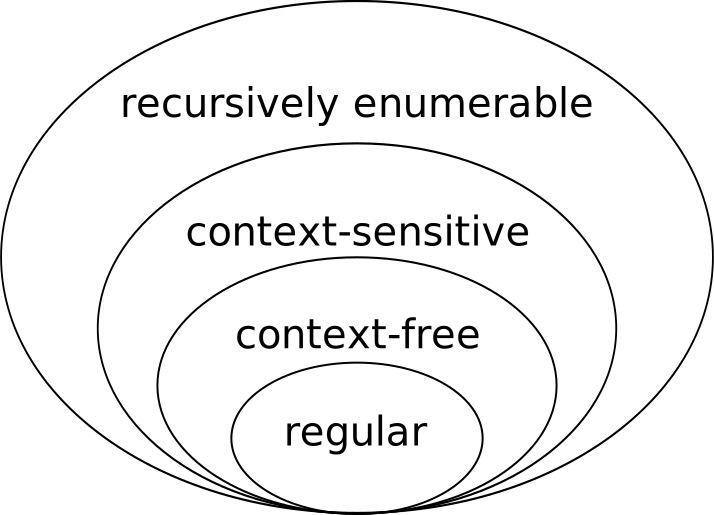
\includegraphics[width=0.2\textwidth]{img/Chomsky-hierarchy.svg}
%\caption{\label{fig:your-figure}Professor of Linguistics (Emeritus) at MIT, Cambridge}
%\end{figure}

\end{frame}

% --------------------------------------------------------------------- %
\begin{frame}{Limiting conditions}

For all production rules $\forall (\alpha \rightarrow \beta)\in P$ it is true:

\begin{block}{First condition}
	\begin{itemize}
		\item $|\alpha| \leq |\beta|$ - they don't decrease length of a word
	\end{itemize}

\end{block}

\begin{block}{Second condition}
	\begin{itemize}
		\item $\alpha\in V_N$ is a nonterminal
		\item $\beta\in V^{+}$ is not empty
	\end{itemize}
\end{block}

\begin{block}{Third condition}
	\begin{itemize}
		\item $\alpha\in V_N$ is a nonterminal
		\item $\beta$ has a form $\beta=a$ or $\beta=aB$ where $a\in V_T, B\in V_N$
	\end{itemize}
\end{block}

\end{frame}

% TODO : put four slides for each type of grammar + limiting condition 

% --------------------------------------------------------------------- %
\begin{frame}{Type-0 : Unrestricted rewriting system}
	
	\begin{block}{Description}
		Type-0 grammar has no limitations (unrestricted)
	\end{block}
	
	\begin{exampleblock}{Valid production rules}
		Production rules have form of $\alpha\rightarrow\beta$, where $\alpha, \beta\in V$
		\begin{itemize}
			\item $aaaA\rightarrow aBb$
			\item $LLQQ\rightarrow LQ$
			\item $S\rightarrow\epsilon$
			\item $C\rightarrow cC$
			\item $D\rightarrow E$
			\item $abcD\rightarrow abc$
		\end{itemize}
	\end{exampleblock}
\end{frame}

% --------------------------------------------------------------------- %

\begin{frame}{Type-0 : Grammar example}
	\begin{block}{Grammar}
		Let $G = (V_N, V_T, P, S)$, where 
		\begin{itemize}
			\item $V_N = \{S, A, B, C, D\}$
			\item $V_T = \{a\}$
			\item \footnotesize$P = \{S\rightarrow ADBC, D\rightarrow DD, DB\rightarrow BEEE, ABE\rightarrow aAB, aABC\rightarrow a\}$
		\end{itemize}
	\end{block}
	
	\begin{block}{Derivations}
		$\textcolor{red}{S}\implies ADBC \implies A\textcolor{red}{DB}C \implies \textcolor{red}{ABE}EEC \implies a\textcolor{red}{ABE}EC \implies aa\textcolor{red}{ABE}C \implies aa\textcolor{red}{aABC} \implies aaa $
	\end{block}
	
	\begin{block}{Language}
		$L(G) = \{a^{m}\}$, where $m=3n \land n \geq 1$
	\end{block}
	
	\begin{exampleblock}{Example sentences}
		$aaa, aaaaaa, aaaaaaaaa, aaaaaaaaaaaa, aaaaaaaaaaaaaaa, ...$
	\end{exampleblock}
\end{frame}

% --------------------------------------------------------------------- %

\begin{frame}{Type-1 : Context-sensitive grammar}
	
	\begin{block}{Description}
		Productions rules of \textit{type-1 grammar} don't decrease the length of the words (i.e. $|\alpha| \leq |\beta|$) during derivations
	\end{block}
	
	\begin{exampleblock}{Valid rules}
		\begin{itemize}
			\item $S \rightarrow \epsilon$
			\item $C \rightarrow cC$
			\item $D \rightarrow E$
			\item $aBc \rightarrow abBc$
		\end{itemize}
	\end{exampleblock}
	
	\begin{alertblock}{Invalid rules}
		\begin{itemize}
			\item $aaaA \rightarrow aBb$
			\item $LLQQ \rightarrow LQ$
			\item $abcD \rightarrow abc$
		\end{itemize}
	\end{alertblock}
	
\end{frame}

% --------------------------------------------------------------------- %

\begin{frame}{Type-1 : Grammar example}
	\begin{block}{Grammar}
		Let $G = (V_N, V_T, P, S)$, where 
		\begin{itemize}
			\item $V_N = \{S, A, B, C, D, E, F\}$
			\item $V_T = \{a, b, c\}$
			\item $P = \{S\rightarrow abC | Ac | Dbc | aEF | aB, A \rightarrow ab, Db \rightarrow ab, B \rightarrow bc, bC \rightarrow bc, F \rightarrow c, Ec \rightarrow bc \}$
		\end{itemize}
	\end{block}
	
	\begin{block}{Derivations}
		\begin{itemize}
			\item $\textcolor{red}{S}\implies a\textcolor{red}{bC} \implies abc$
			\item $\textcolor{red}{S}\implies \textcolor{red}{A}c \implies abc$
			\item $\textcolor{red}{S}\implies aE\textcolor{red}{F} \implies a\textcolor{red}{Ec} \implies abc$
		\end{itemize}
	\end{block}
	
	\begin{exampleblock}{Language and example sentence}
		$L(G) = \{abc\}$
	\end{exampleblock}

\end{frame}

% --------------------------------------------------------------------- %

\begin{frame}{Type-2 : Context-free grammar}
	
	\begin{block}{Description}
		Rules $A \rightarrow \beta$ in context-free grammar have one variable (nonterminal) on the left hand side ($A\in V_N$) and they derive into any word ($\beta \in V^*$)
	\end{block}
	
	\begin{exampleblock}{Valid rules}
		\begin{itemize}
			\item $S \rightarrow \epsilon$
			\item $C \rightarrow cC$
			\item $D \rightarrow E$
			\item $F \rightarrow abcdef$
		\end{itemize}
	\end{exampleblock}
	
	\begin{alertblock}{Invalid rules}
		\begin{itemize}
			\item $aaaA \rightarrow aBb$
			\item $LLQQ \rightarrow LQ$
			\item $aBc \rightarrow abefBc$			
		\end{itemize}
	\end{alertblock}
	
\end{frame}

% --------------------------------------------------------------------- %

\begin{frame}{Type-2 : Grammar example}
	\begin{block}{Grammar}
		Let $G = (V_N, V_T, P, S)$, where 
		\begin{itemize}
			\item $V_N = \{S, A, B\}$
			\item $V_T = \{a, b\}$
			\item $P = \{S\rightarrow aSB, S\rightarrow A, A \rightarrow ab, B\rightarrow b\}$
		\end{itemize}
	\end{block}
	
	\begin{block}{Derivations}
		$\textcolor{red}{S}\implies a\textcolor{red}{S}B \implies aaSB\textcolor{red}{B} \implies aaS\textcolor{red}{B}b \implies aa\textcolor{red}{S}bb \implies aaabbb$
	\end{block}
	
	\begin{block}{Language}
		$L(G) = \{a^nb^n\}$, where $n\geq 1$
	\end{block}
	
	\begin{exampleblock}{Example sentences}
		$ab, aabb, aaabbb, aaaabbbb, aaaaabbbbb, aaaaaabbbbbb, ...$
	\end{exampleblock}
\end{frame}

% --------------------------------------------------------------------- %

\begin{frame}{Type-3 : Regular grammar}
	
	\begin{block}{Description}
		Rules in regular grammar have form of $A\rightarrow a$ and $A\rightarrow aB$ (right recursion) or $A\rightarrow Ba$ (left recursion), where $A,B\in V_N$ and $a\in V_T$
	\end{block}
	
	\begin{exampleblock}{Valid rules}
		\begin{itemize}
			\item $C \rightarrow cD$
			\item $D \rightarrow Dc$
			\item $S \rightarrow b$
		\end{itemize}
	\end{exampleblock}
	
	\begin{alertblock}{Invalid rules}
		\begin{itemize}
			\item $S \rightarrow \epsilon$
			\item $D \rightarrow E$
			\item $aBc \rightarrow abefBc$			
			\item $F \rightarrow abcdef$			
		\end{itemize}
	\end{alertblock}
	
\end{frame}

% --------------------------------------------------------------------- %

\begin{frame}{Grammar example -- regular}
	
	\begin{block}{Grammar}
		Let $G = (V_N, V_T, P, S)$, where 
		\begin{itemize}
			\item $V_N = \{S, B\}$
			\item $V_T = \{a,b\}$
			\item $P = \{S \rightarrow aB, B \rightarrow bS, B \rightarrow b\}$
		\end{itemize}
	\end{block}
	
	\begin{block}{Derivation}
		$\textcolor{red}{S} \implies a\textcolor{red}{B} \implies ab\textcolor{red}{S} \implies aba\textcolor{red}{B} \implies abab\textcolor{red}{S} \implies ababa\textcolor{red}{B} \implies ...$
	\end{block}
	
	\begin{block}{Language}
		$L(G) = \{(ab)^n\}$, where $n\geq 1$.
	\end{block}
	
	\begin{exampleblock}{Example sentences}
		$ab, abab, ababab, abababab, ababababab, abababababab, ...$
	\end{exampleblock}
	
\end{frame}

\begin{frame}{Normal forms}

\end{frame}

\begin{frame}{Derivation trees}
	Also : tree diagrams, phrase markers. For regular and context-free grammars.
\end{frame}

% --------------------------------------------------------------------- %

\begin{frame}{Grammar examples}
	\begin{block}{Grammar}
		Let $G = (V_N, V_T, P, S)$, where 
		\begin{itemize}
			\item $V_N = \{S\}$
			\item $V_T = \{a,b\}$
			\item $P = \{\textcolor{red}{S \rightarrow aS} \lor \textcolor{blue}{S \rightarrow Sa}, S \rightarrow b\}$
		\end{itemize}
	\end{block}
	
	\begin{block}{Derivations}
		$\textcolor{red}{S}\implies a\textcolor{red}{S}\implies aa\textcolor{red}{S} \implies aaa\textcolor{red}{S} \implies aaaa\textcolor{red}{S} \implies aaaaa\textcolor{red}{S} \implies ...$
		\\ $\textcolor{blue}{S}\implies \textcolor{blue}{S}a\implies \textcolor{blue}{S}aa \implies \textcolor{blue}{S}aaa \implies \textcolor{blue}{S}aaaa \implies \textcolor{blue}{S}aaaaa \implies ...$
	\end{block}
	
	\begin{block}{Language}
		$L(G) = \{a^{n}b\}$, where $n \geq 0$
	\end{block}
	
	\begin{exampleblock}{Example sentences}
		$b, ab, aab, aaab, aaaab, aaaaab, aaaaaab, aaaaaaab, aaaaaaaab, ...$
	\end{exampleblock}
\end{frame}

\begin{frame}{Grammar example: \textit{mirror language}}
	\begin{block}{Grammar}
		Let $G = (V_N, V_T, P, S)$, where 
		\begin{itemize}
			\item $V_N = \{S\}$
			\item $V_T = \{a,b\}$
			\item $P = \{S \rightarrow aSa, S \rightarrow bSb, S \rightarrow aa, S \rightarrow bb\}$
		\end{itemize}
	\end{block}
	
	\begin{block}{Derivations}
		$\textcolor{red}{S}\implies a\textcolor{red}{S}a \implies ab\textcolor{red}{S}ba \implies abb\textcolor{red}{S}bbs \implies abba\textcolor{red}{S}abba \implies ...$
	\end{block}
	
	\begin{block}{Language}
		$L(G) = \{ww^R\}$, where $w^R$ represents reflection of $w$, and $|w|\geq1$. This language $L(G)$ is called a \textit{mirror language}.
	\end{block}
	
	\begin{exampleblock}{Example sentences}
		$aa, bb, aaaa, abba, baab, bbbb, abaaba, baaaab, abbbba, babbab, aaaaaa...$
	\end{exampleblock}
\end{frame}

\begin{frame}{Grammar example}
	\begin{block}{Grammar}
		Let $G = (V_N, V_T, P, S)$, where 
		\begin{itemize}
			\item $V_N = \{S, E, F\}$
			\item $V_T = \{a,b,c,d\}$
			\item $P = \{S \rightarrow ESF, S \rightarrow EF, E \rightarrow ab, F \rightarrow cd\}$
		\end{itemize}
	\end{block}
	
	\begin{block}{Derivations}
		\small$\textcolor{red}{S} \implies E\textcolor{red}{S}F \implies EE\textcolor{red}{S}FF \implies EEE\textcolor{red}{S}FFF \implies E^{n-1}\textcolor{red}{S}F^{n-1} \implies E^nF^n$
	\end{block}
	
	\begin{block}{Language}
		$L(G) = \{(ab)^n(cd)^n\}$, where $n\geq 1$.
	\end{block}
	
	\begin{exampleblock}{Example sentences}
		$abcd, ababcdcd, abababcdcdcd, ababababcdcdcdcd, ...$
	\end{exampleblock}
\end{frame}

\begin{frame}{Grammar example}
	\begin{block}{Grammar}
		Let $G = (V_N, V_T, P, S)$, where 
		\begin{itemize}
			\item \small$V_N = \{S, E, F\}$
			\item \small$V_T = \{a,b,c,d\}$
			\item \small$P = \{S \rightarrow ESF, S \rightarrow abcd, Ea \rightarrow aE, dF \rightarrow Fd, Eb \rightarrow abb, cF \rightarrow ccd\}$\normalsize
		\end{itemize}
	\end{block}
	% mark red active symbols !!
	\begin{block}{Derivations}
		\footnotesize$\textcolor{red}{S} \implies E\textcolor{red}{S}F \implies \textcolor{red}{Ea}bcdF \implies aEbc\textcolor{red}{dF} \implies a\textcolor{red}{Eb}cFd \implies aabbc\textcolor{red}{Fd} \implies aabbccdd$ 
	\end{block}
	
	\begin{block}{Language}
		$L(G) = \{a^nb^nc^nd^n\}$, where $n \geq 2$.
	\end{block}
	
	\begin{exampleblock}{Sentences}
		$aabbccdd, aaabbbcccddd, aaaabbbbccccdddd, aaaaabbbbbcccccddddd, ...$
	\end{exampleblock}
	
\end{frame}

%\subsection{Notation}
\begin{frame}{Language and grammar}
Two common tasks:

\begin{itemize}
	\item Check if language is legal (accepted by the grammar) -- trace all the applicable rules (derive it language from the start symbol) or... use corresponding automaton!
	\item Generate language from grammar -- start from \textit{start symbol}, go through all applicable rules
\end{itemize}
\end{frame}

% --------------------------------------------------------------------- %
\begin{frame}[fragile]{Backus-Naur form (BNF)}

\begin{block}{Backus-Naur form (BNF)}
Notation technique for \textit{context-free grammars}. Frequently used to describe syntax of \textit{programming languages}, \textit{document formats} etc.
\end{block}


\begin{block}{Syntax}
\begin{verbatim}
                 <term> ::= __expression__
\end{verbatim}
\vskip -0.5cm
\begin{itemize}
\item \verb|<term>| is a \textit{nonterminal}
\item \verb|__expression__| is a sequence of one or more terminal and/or nonterminal symbols separated by vertical line \verb$|$
\item Terminal symbols: \verb|a|, \verb|b|, \verb|c|, \verb|A|, \verb|0|, \verb|1|, \verb|2| etc.
\item Nonterminal symbols: \verb|<digit>|, \verb|<postal-code>| etc.
\end{itemize}
\end{block}

\end{frame}

% --------------------------------------------------------------------- %
\begin{frame}[fragile]{Backus-Naur form (BNF)}

\begin{block}{Meta-symbols}
\begin{itemize}
\item $::=$ -- production rule definition
\item $|$ -- rule alternative
\item $< >$ -- nonterminals
\item $""$ -- literal
\item $<EOL>$ -- End Of Line
\end{itemize}
\end{block}

\begin{exampleblock}{Examples}
\small
\begin{verbatim}
<digit> ::= 0 | 1 | 2 | 3 | 4 | 5 | 6 | 7 | 8 | 9
<postal-code> ::= <digit> <digit> <digit> <digit> <digit>
\end{verbatim}
\end{exampleblock}

\end{frame}

% --------------------------------------------------------------------- %
\begin{frame}[fragile]{BNF example : Palindrome}

\begin{exampleblock}{Palindrome grammar}
\begin{verbatim}
<letter>     ::= a | b | c | ... | y | z
<palindrome> ::= <letter> |
<palindrome> ::= a <palindrome> a | b <palindrome> b |
                 c <palindrome> c | d <palindrome> d | 
                 e <palindrome> e | ...
                                  | z <palindrome> z
\end{verbatim}
\end{exampleblock}

\begin{exampleblock}{Results}
\begin{verbatim}
a
bb
bab
pop
hannah
\end{verbatim}
\end{exampleblock}

\end{frame}

% --------------------------------------------------------------------- %
\begin{frame}[fragile]{BNF example : Postal address}
\begin{exampleblock}{Postal address grammar}\small
\begin{verbatim}
<postal-address> ::= <name-part> <street-address> <zip-part>
<name-part> ::= <first-name> <last-name> <EOL> 
<street-address> ::= <number> <street-name> <apt-num> <EOL>
<zip-part> ::= <postal-code> <town-name> <EOL>
<apt-num> ::= <number> | ""
\end{verbatim}
\end{exampleblock}
\end{frame}

% --------------------------------------------------------------------- %
%\begin{frame}{Extended Backus-Naur form (EBNF)}
%\end{frame}

\section{Parsing}

\subsection{Methods}

\subsection{Tools}

\section{ANTLR}

% --------------------------------------------------------------------- %
\begin{frame}{ANTLR v4}
	
\begin{block}{Parser generator}
	content...
\end{block}	
	
\begin{block}{ANTLR}
A parser generator which allows to:
\begin{itemize}
	\item 
\end{itemize}
\end{block}

\begin{exampleblock}{Usages}
	\begin{itemize}
		\item Twitter search queries are parsed using ANTLR
		\item Lex Machina\footnote{lexmachina.com} extracts informations from legal texts using ANTLR
	\end{itemize}
\end{exampleblock}
	
\end{frame}

\begin{frame}[fragile]{ANTLR syntax (I)}

	\begin{minipage}[t]{0.3\textwidth}
		\begin{exampleblock}{Grammar structure}		
			\footnotesize
			\begin{lstlisting}
				grammar ANY_NAME;
				options {...}
				import ... ;
				tokens {...}
				channels {...}
				@actionName{...}
				// lexer rules
				LEXER_RULE1
				LEXER_RULE2
				// parser rules
				parser_rule1
				parser_rule2			
			\end{lstlisting}
		\end{exampleblock}
	\end{minipage}
	\noindent\hfill
	\begin{minipage}[t]{0.65\textwidth}
		\begin{block}{Grammar properties}
			\begin{itemize}
				\item Each section can be specified in any order
				\item Only one definition for sections: \textit{options}, \textit{imports}, \textit{tokens}
				\item The header and at least one rule are mandatory
			\end{itemize}
		\end{block}

			\begin{alertblock}{Reserved keywords}
				\textit{import, fragment, lexer, parser, grammar, returns, locals, throws, catch, finally, mode, options, tokens}
			\end{alertblock}
			
	\end{minipage}
		\begin{alertblock}{Grammar file}
			The file name with grammar \textit{ANY\_NAME} must be called \textit{ANY\_NAME.g4}
		\end{alertblock}	

\end{frame}

\begin{frame}{Lexer vs parser}
	
\begin{figure}
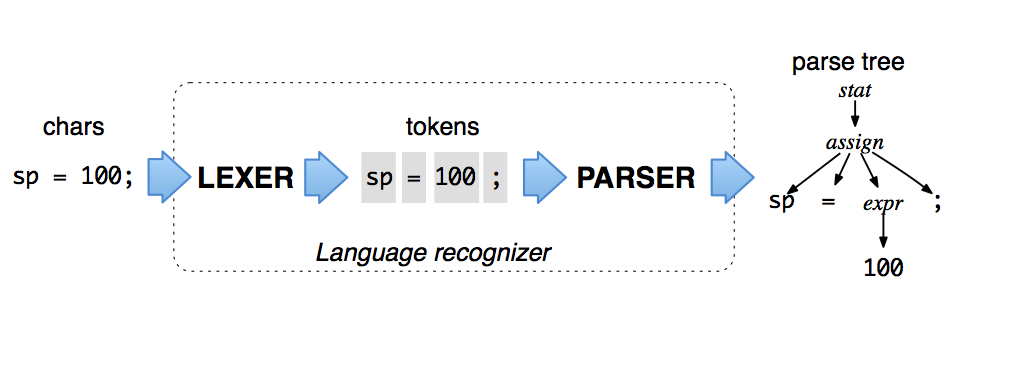
\includegraphics[width=\textwidth]{img/lexer_parser_scheme}
\vskip -1.2cm
\caption{\label{fig:your-figure}Caption goes here\footnotemark}
\end{figure}
	
	
	
%	Lexical analysis converts a sequences of characters into a sequence of tokens (strings with meanings).
	
%	\begin{block}{Parser}
%		Performs \textit{lexical analysis} which is classification of sequence of symbols into lexemes (tokens). Single characters are symbols for lexer. Lexer understand regular grammar (Chomsky's level 3).
%	\end{block}
	
	\begin{block}{Lexer}
		Tokens (terminal symbols with semantics) are symbols for the parser. Parser understands context-free grammar (Chomsky's level 2).
	\end{block}

\footnotetext[1]{\tiny From ANTLR4 on-line documentation}

\end{frame}

\begin{frame}{ANTLR syntax (II)}
	\begin{table}[H]
		\begin{tabular}{c|c}
			\textbf{Syntax} & \textbf{Description} \\
			\hline
			$x$ & Match token, rule or subrule $x$ \\
			$x y ....z$ & Match a sequence of elements \\
			$(...|...|...)$ & Sub-rule with multiple alternatives \\
			$x?$ & Match $x$ or skip it \\
			$x*$ & Match $x$ zero or more times \\
			$x+$ & Match $x$ one or more times \\
			$r: ...$ & Define rule $r$ \\
			$r: (...|...|...)$ & Define rule $r$ with multiple alternatives
		\end{tabular}
	\end{table}
\end{frame}

\begin{frame}[fragile]{ANTLR patterns}
	\begin{table}[H]
		\begin{tabular}{c|c}
			\textbf{Pattern name} & \textbf{Examples} \\
			\hline
			Sequence & \verb|'[' INT+ ']'|\\
			Sequence with terminator & \verb|(statement ';')*| \\
			Sequence with separator & \verb|( expr (',' expr)*)?| \\
			Choice & \verb^type : 'int' | 'float'^\\
			Token dependency & \verb|ID '[' expr ']'| \\
			Nested phrase & \verb^expr : '(' expr ')' | ID^
		\end{tabular}
	\end{table}
\end{frame}

\begin{frame}{Action and semantic predicate}
	
\end{frame}

\begin{frame}[fragile]{First grammar}
	\begin{exampleblock}{Simple grammar (Hello.g4)}
		\begin{verbatim}
// define a grammar called Hello
grammar Hello;
// match lower-case identifiers
ID : [a-z]+;
// skip spaces, tabs, newlines, \r (Windows)
WS : [ \t\r\n]+ -> skip;
// match keyword hello followed by an identifier
r : 'hello' ID;
		\end{verbatim}
	\end{exampleblock}
\end{frame}

\begin{frame}[fragile]{Nested arrays}
	
	\begin{exampleblock}{Nested arrays grammar (ArrayInit.g4)}
		\begin{verbatim}
			grammar ArrayInit;
			// matches at least one comma-separated value between {...}
			init : '{' value (',' value)* '}';
			// A value can be either a nested array or an integer (INT)
			value : init | INT;
			// define token INT as one or more digits
			INT : [0-9]+;
			WS : [ \t\r\n]+ -> skip;
		\end{verbatim}
	\end{exampleblock}
				// parser rules start with lowercase letters, lexer rules with uppercase
\end{frame}

% TODO: use package listings
\begin{frame}[fragile]{Parser tester}
	\begin{exampleblock}{Parser}
		\begin{lstlisting}[basicstyle=\tiny, language=Java]
			import org.antlr.v4.runtime.*;
			import org.antlr.v4.runtime.tree.*;
			
			public class Test { 
			    public static void main(String[] args) throws Exception { 
			        // create a CharStream that reads from standard input 
			        ANTLRInputStream input = new ANTLRInputStream(System.in);
			        // create a lexer that feeds off of input 
			        CharStream ArrayInitLexer lexer = new ArrayInitLexer(input);
			        // create a buffer of tokens pulled from the lexer 
			        CommonTokenStream tokens = new CommonTokenStream(lexer);
			        // create a parser that feeds off the tokens buffer 
			        ArrayInitParser parser = new ArrayInitParser(tokens);
			        ParseTree tree = parser.init();
			        System.out.println(tree.toStringTree(parser));
			    } 
			}
			
		\end{lstlisting}
	\end{exampleblock}
\end{frame}

\begin{frame}[fragile]{Calculator}
\begin{lstlisting}[style=ANTLR]
grammar Expr;

prog: stat+;
stat: expr NEWLINE
    | ID '=' expr NEWLINE
    | NEWLINE;

expr: expr ('*'|'/') expr
    | expr ('+'|'-') expr
    | INT
    | ID
    | '(' expr ')';

ID : [a-zA-Z]+;
INT : [0-9]+;
// return newlines to parser (is end-statement signal)
NEWLINE:'\r'? '\n';
WS : [ \t]+ -> skip;
\end{lstlisting}
\end{frame}

\begin{frame}{Generated parser}
	zawartość...
\end{frame}

\begin{frame}{Generated lexer}
	zawartość...
\end{frame}

\begin{frame}{Generated tree visitor}
	zawartość...
\end{frame}

\begin{frame}{Generated tree listener}
	zawartość...
\end{frame}

\begin{frame}{Importing grammars}
	show two files : lexer \& grammar
\end{frame}

\begin{frame}{ANTLR caveats}
	\begin{itemize}
		\item Lexer/Parser rules order matter
		\item 
	\end{itemize}
\end{frame}

% Commands to include a figure:
%\begin{figure}
%\includegraphics[width=\textwidth]{your-figure's-file-name}
%\caption{\label{fig:your-figure}Caption goes here.}
%\end{figure}


\end{document}
